\chapter{Methodology}
This chapter covers the various methodologies that were implemented in this 
project. It takes a look at the different types of research methodologies that 
were used such as Qualitative Research, Quantitative Research, and Mixed Methods
Research and the different types of software development methodologies that were
used such as Test Driven Development, Continuous Delivery, Extreme Programming, 
etc. and why each was chosen. Other areas also covered in this chapter include
meetings, project management, development tools, source control, and testing.

\section{Research Methodology}
The research methodology that was used in this project was a Mixed Methods 
Research methodology, using a mix of both Qualitative Research and Quantitative 
Research. Qualitative research approaches are employed across many academic 
disciplines and is useful at an individual level. Qualitative data collection
methods vary using unstructured or semi-structured techniques.
\par
\medskip
Various data collection tools were used for gathering data such as

\section{Software Development Methodology}
\begin{center}
    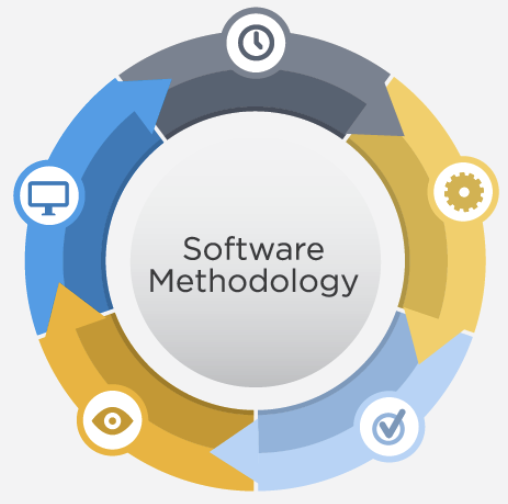
\includegraphics[width=8cm,height=3.3cm,keepaspectratio]{images/software_methodology}
    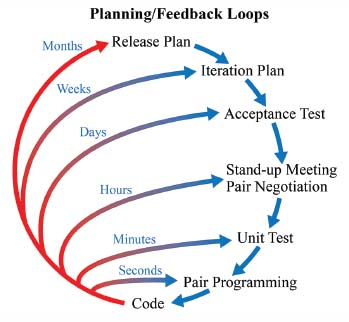
\includegraphics[width=8cm,height=3.3cm,keepaspectratio]{images/xp}
\end{center}
\par
The software development methodology that was used in this project was Extreme 
Programming (XP). Extreme Programming is a software development methodology 
designed to improve the quality of software and its ability to properly adapt to
the changing needs of the customer or client. While there was no customer or 
client for this project, this methodology was still applicable. 
\par
\medskip
\begin{center}
    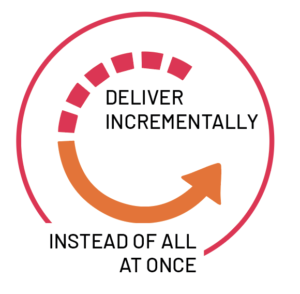
\includegraphics[width=8cm,height=3.3cm,keepaspectratio]{images/agile}
\end{center}
It is a form of Agile software development. The Agile methodology was developed 
as a response to growing frustrations with Waterfall and other highly 
structured, inflexible methodologies. This approach is designed to accommodate 
change and the need to produce software faster. Similar to other Agile methods 
of development, Extreme Programming aims to provide iterative and frequent small
releases throughout the project, allowing both team members and customers to 
examine and review the project’s progress throughout the entire SDLC (Software
Development Life Cycle). 
\par
\medskip
It became clear early on that the Agile methodology would be the most suitable 
methodology to use for this project as the Agile Methodology allows for 
incremental development, changing requirements, prototyping, and sustainable 
development. As there would be weekly meetings with the project supervisor, 
being able to show and discuss the progress of the project would be a bonus. 

\section{Meetings}
Project meetings were held weekly for the duration of the project with the
project supervisor. The majority of the meetings consisted of:
\begin{itemize}
    \item Project progress updates.
    \item Feedback on progress.
    \item Planning of the next development iteration.
    \item Discussions on possible additional features that could be
    incorporated.
    \item Q&A on various project elements.
\end{itemize}
\par
\medskip
Initial project meetings were more focused on brainstorming possible projects
that could be developed. The first two weeks comprised of research, whereby 
possible projects ideas, appropriate technologies, and a project timeline were
developed.

\section{Development Tools}
\begin{center}
    
\includegraphics[width=8cm,height=3.3cm,keepaspectratio]{images/vscode}
\end{center}
The main Integrated Development Environment used throughout the project was 
Visual Studio Code. Visual Studio Code is a source-code editor developed by 
Microsoft for Windows, Linux and mac OS. It includes support for debugging, 
embedded Git control and GitHub, syntax highlighting, intelligent code 
completion, snippets, and code refactoring. 
\par
\bigskip
Visual Studio Code is based on Electron, a framework which is used to develop
Node.js applications for the desktop running on the Blink layout engine. Visual 
Studio Code is a source code editor that can be used with a variety of 
programming languages, including Java, JavaScript, Go, Node.js and C++.

\section{Source Control}
\begin{center}
    
\includegraphics[width=8cm,height=3.3cm,keepaspectratio]{images/github}
\end{center}

Source control (or version control) is the practice of tracking and managing
changes to code. GitHub provides hosting for software development version
control using Git. Git is an open-source distributed source code management
system.

\subsubsection{Advantages}
There are a number of advantages to using Git:

\begin{itemize}
    \item \textbf{Distributed Development} - Git is a distributed version
    control system. Instead of a working copy, each developer gets their own 
    local repository, complete with a full history of commits. Having a full 
    local history makes Git fast, since it means you don’t need a network 
    connection to create commits, inspect previous versions of a file, or 
    perform diffs between commits.
    \item \textbf{Faster Release Cycle} - As a result of feature branches,
    distributed development, pull requests, etc. is a faster release cycle. This
    facilitates an agile workflow, encouraging developers to share smaller 
    changes more frequently. This results in changes get pushed down the 
    development pipeline faster
    \item \textbf{Testing} - The main type of software testing development 
    process used throughout the project was Test-driven development (TDD). 
    Several different types of testing was used throughout in conjunction, such 
    as Integration Testing, Unit Testing, System Testing, Performance Testing, 
    etc. Several tools were used to aid in this, which included Postman, ... TDD
    allows for continuous testing to happen alongside the development of the 
    project.
\end{itemize}
\par
\medskip
\subsubsection{Disadvantages}
Git is a very well-designed tool and, as such, has very few disadvantages:

\begin{itemize}
    \item \textbf{Pricing} - Some of GitHub features, as well as features on 
    other online repositories, are locked behind a SaaS paywall. If you have a 
    large team, this can add up fast. Those who already have a dedicated IT team
    and their own internal servers are often better off using their own internal
    git for cost reasons, but for most, the cost isn’t outrageous.
    \item \textbf{Security} - GitHub does offer private repositories, but this
    isn’t necessarily perfect for many. For high value intellectual property, 
    you’re putting all of this in the hands of GitHub as well as anyone who has 
    a login, which like many sites has had security breaches before and is 
    targeted constantly. In addition, some clients/employers will only allow 
    code on their own secure internal Git as a matter of policy.
\end{itemize}

The above mentioned testing processes suited this type of project as there were
many different iterations of the project. Using testing processes such as 
Integration Testing, Unit Testing, System Testing, etc. ensured new and old code
worked with each and every iteration of the project.
\par
\medskip
\par
\medskip
\begin{center}
    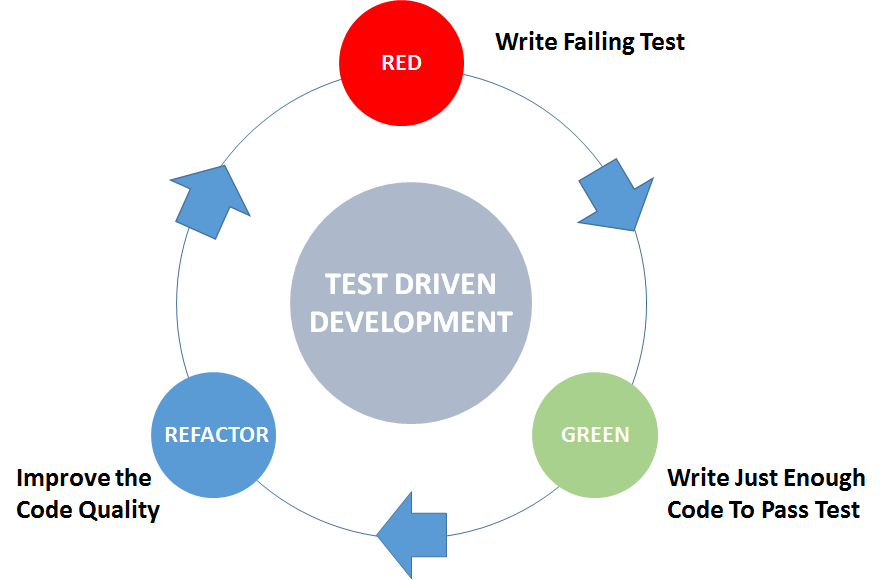
\includegraphics[width=8cm,height=3.3cm,keepaspectratio]{images/tdd}
\end{center}